% !TEX root = ../../thesis.tex

\section{Numerics}
\label{sec:nums}

Proving quantities are conserved is a great way of theoretically verifying our results are correct. However, in practicality, numerical analysts are interested in this area of mathematics to create more precise numerical schemes. We shall now show that normal numerical schemes sometimes provide non-realistic solutions and how we can produce more realistic results.\\

\noindent
We shall take the standard Euler equations as a simplistic example to show our point. Consider the following Euler equation.
$$ \pd {\vec u} t + ({\vec u} \cdot\nab){\vec u} = 0. $$
We can run a Crank-Nicholson scheme on this. It is well known that Crank-Nicholson is symplectic; that is, it preserves the symplectic form. Further, this means that it conserves energy. These schemes can be adapted to conserve other quantities. We consider a finite element scheme with a cubed $50\times 50$ grid with order $2$ Lagrange elements to motivate these. We set an initial condition of,
$$ u_0(x,\, y) = \left( -\cos \left( \frac{\pi x}{2} \right)\sin \left( \frac{\pi x}{2} \right),\, \sin\left( \frac{\pi x}{2} \right)\cos \left( \frac{\pi y}{2} \right) \right), $$
and Neumann boundary conditions. The finite element scheme solves the spatial steps, and we use a Crank-Nicholson for the temporal steps. Hence, our scheme is,
$$ \frac{{\vec u}^{n+1} - {\vec u}^n}{\D t} = \frac{1}{2}\left( \left({\vec u}^{n+1} \cdot \nab\right){\vec u}^{n+1} + \left({\vec u}^{n} \cdot \nab\right){\vec u}^{n}\right). $$
We notice that we haven't produced a weak form of the equation. This is due to the Euler equations being unstable with weak forms.
This produces the following simulation in Figure \ref{fig:Sim}.

\begin{figure*}[!ht]
  \centering
  \begin{subfigure}[b]{0.475\textwidth}
      \centering
      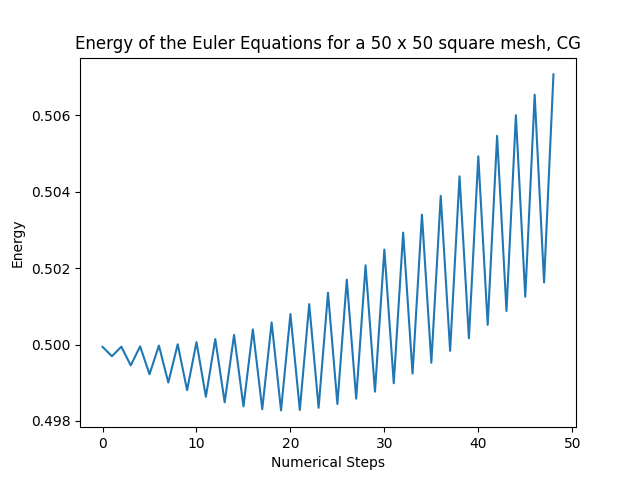
\includegraphics[width=\textwidth]{./img/energy}
      \caption[Network2]%
      {{\small t = 0.25}}
      \label{fig:energy}
  \end{subfigure}
  \hfill
  \begin{subfigure}[b]{0.475\textwidth}
      \centering
      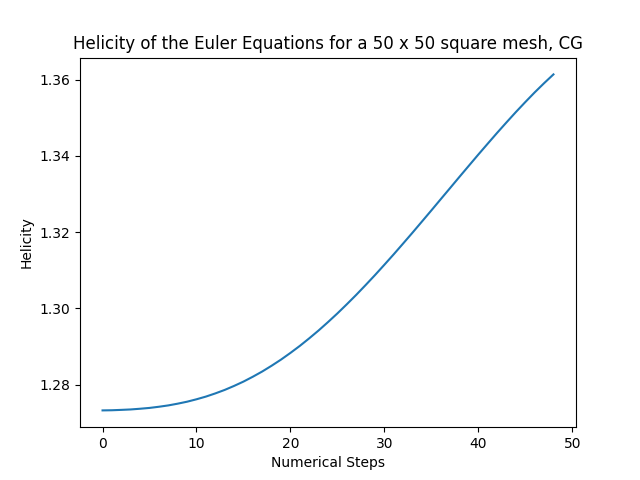
\includegraphics[width=\textwidth]{./img/helicity}
      \caption[]%
      {{\small t = 0.5}}
      \label{fig:helcity}
  \end{subfigure}
  \caption{Conservation of Helicity and Energy in the FEM Scheme}
  \label{fig:conservation}
\end{figure*}

\noindent
We can also consider the conserved quantities. In this system, we will consider the total energy and enstrophy,
$$ E = \int_M |\vec u|^2\mu \qquad H = \int_M \vec u \cdot \mathrm{rot} \vec u\mu . $$

\begin{figure*}
    \centering
    \begin{subfigure}[b]{0.475\textwidth}
        \centering
        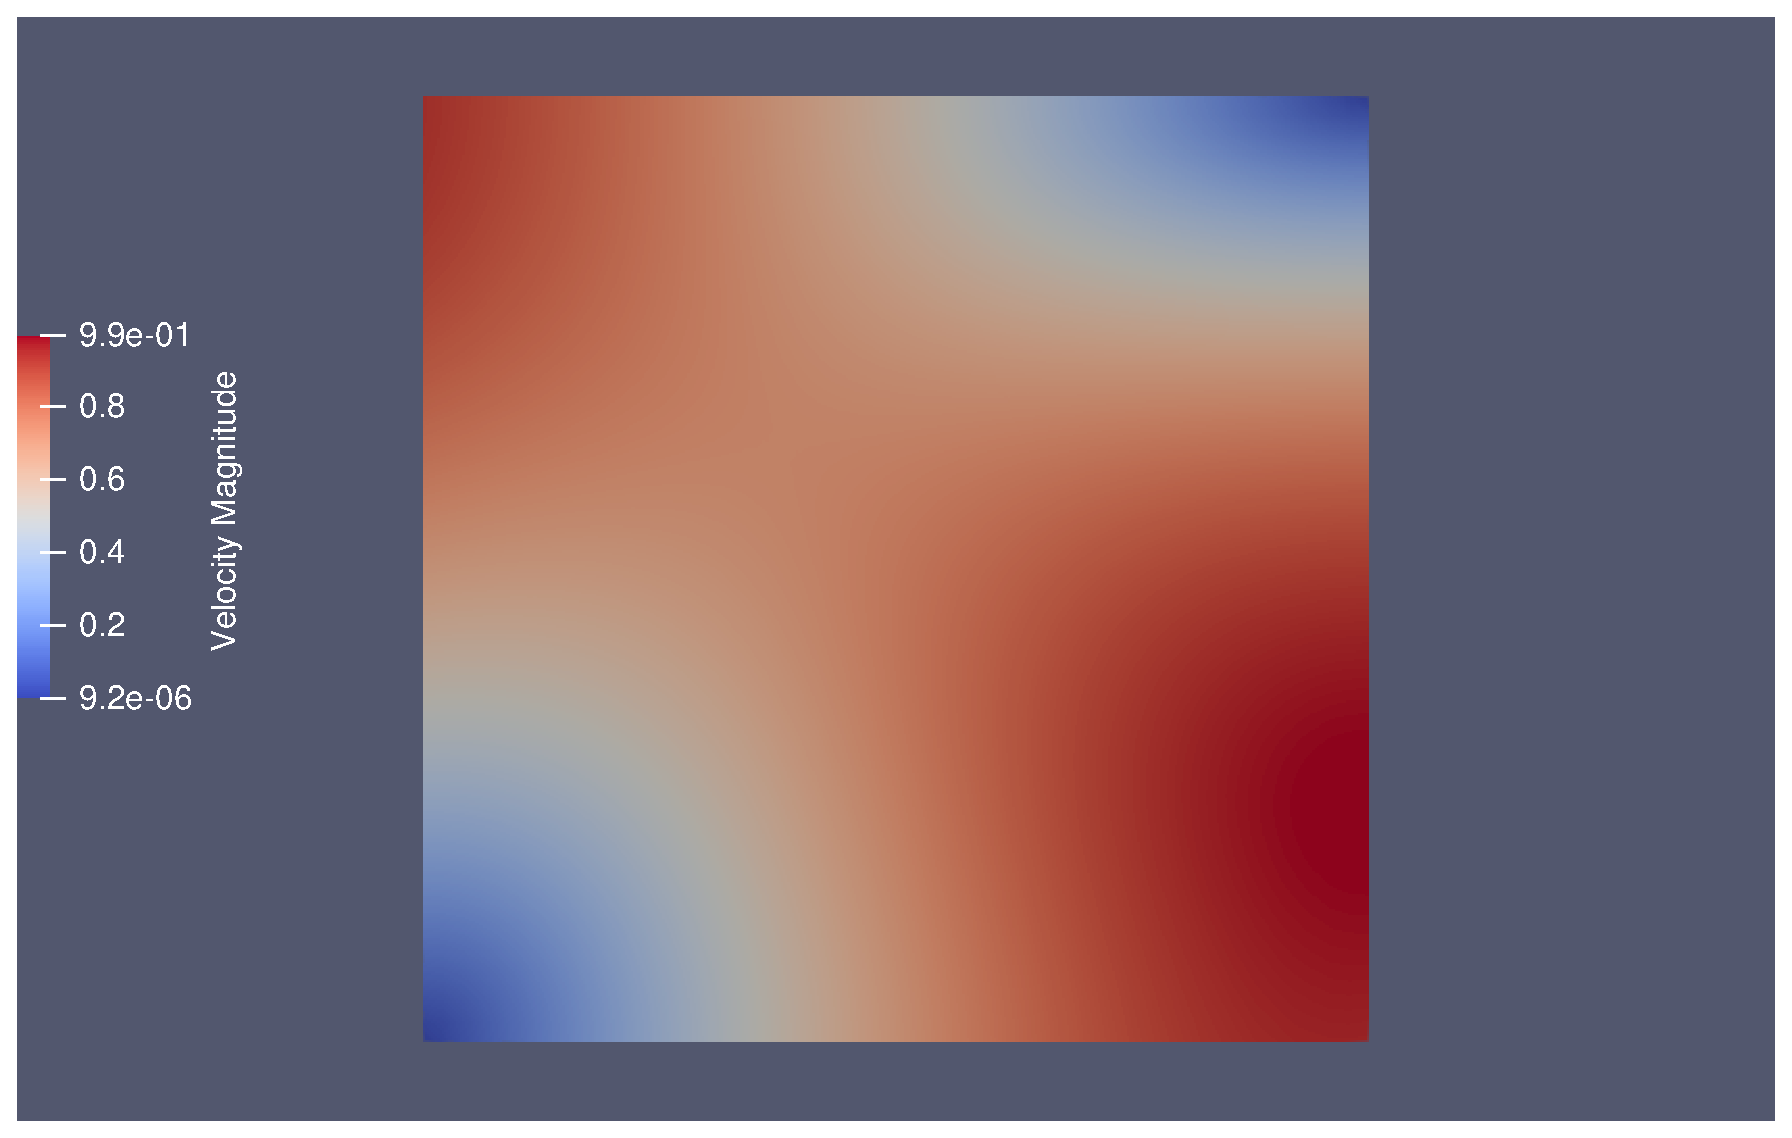
\includegraphics[trim={5cm 0 5cm 0}, clip,width=\textwidth]{./img/25.eps}
        \caption[Network2]%
        {{\small t = 0.25}}
        \label{fig:0.25}
    \end{subfigure}
    \hfill
    \begin{subfigure}[b]{0.475\textwidth}
        \centering
        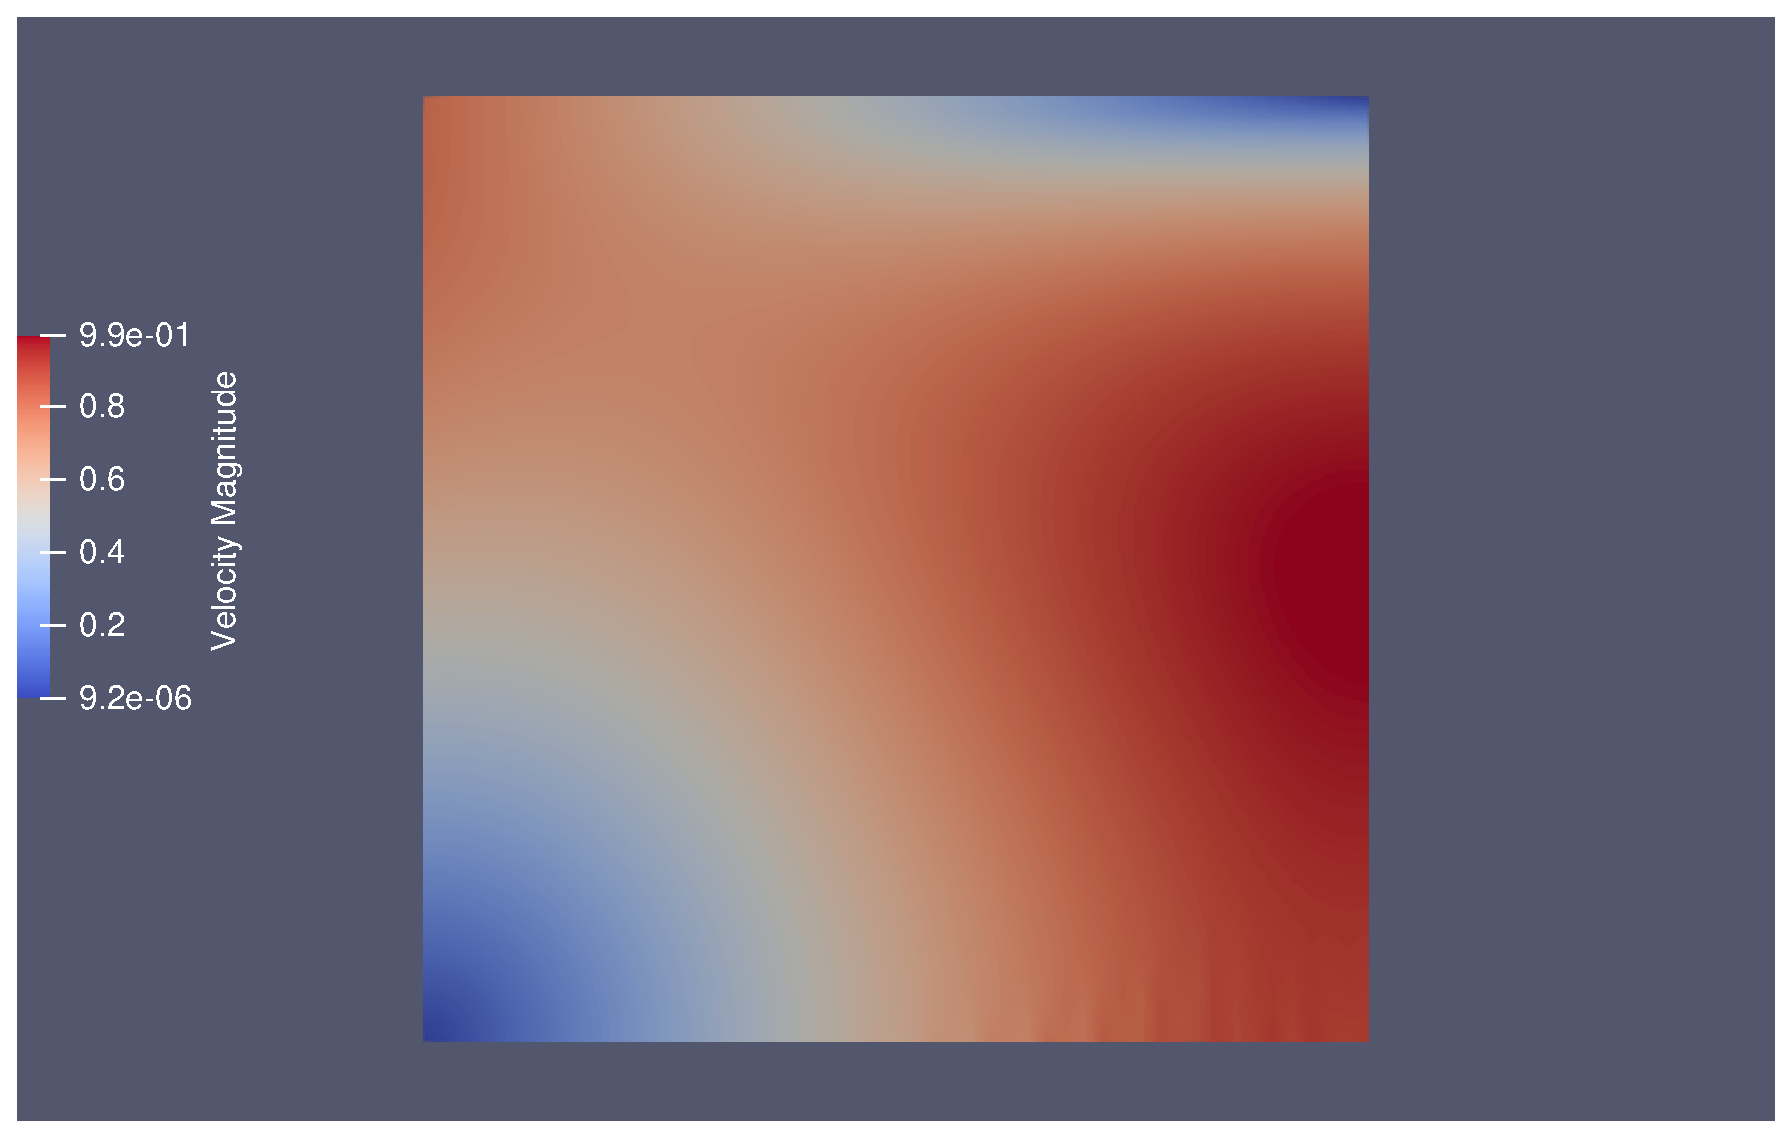
\includegraphics[trim={5cm 0 5cm 0}, clip,width=\textwidth]{./img/50.eps}
        \caption[]%
        {{\small t = 0.5}}
        \label{fig:0.5}
    \end{subfigure}
    \vskip\baselineskip
    \begin{subfigure}[b]{0.475\textwidth}
        \centering
        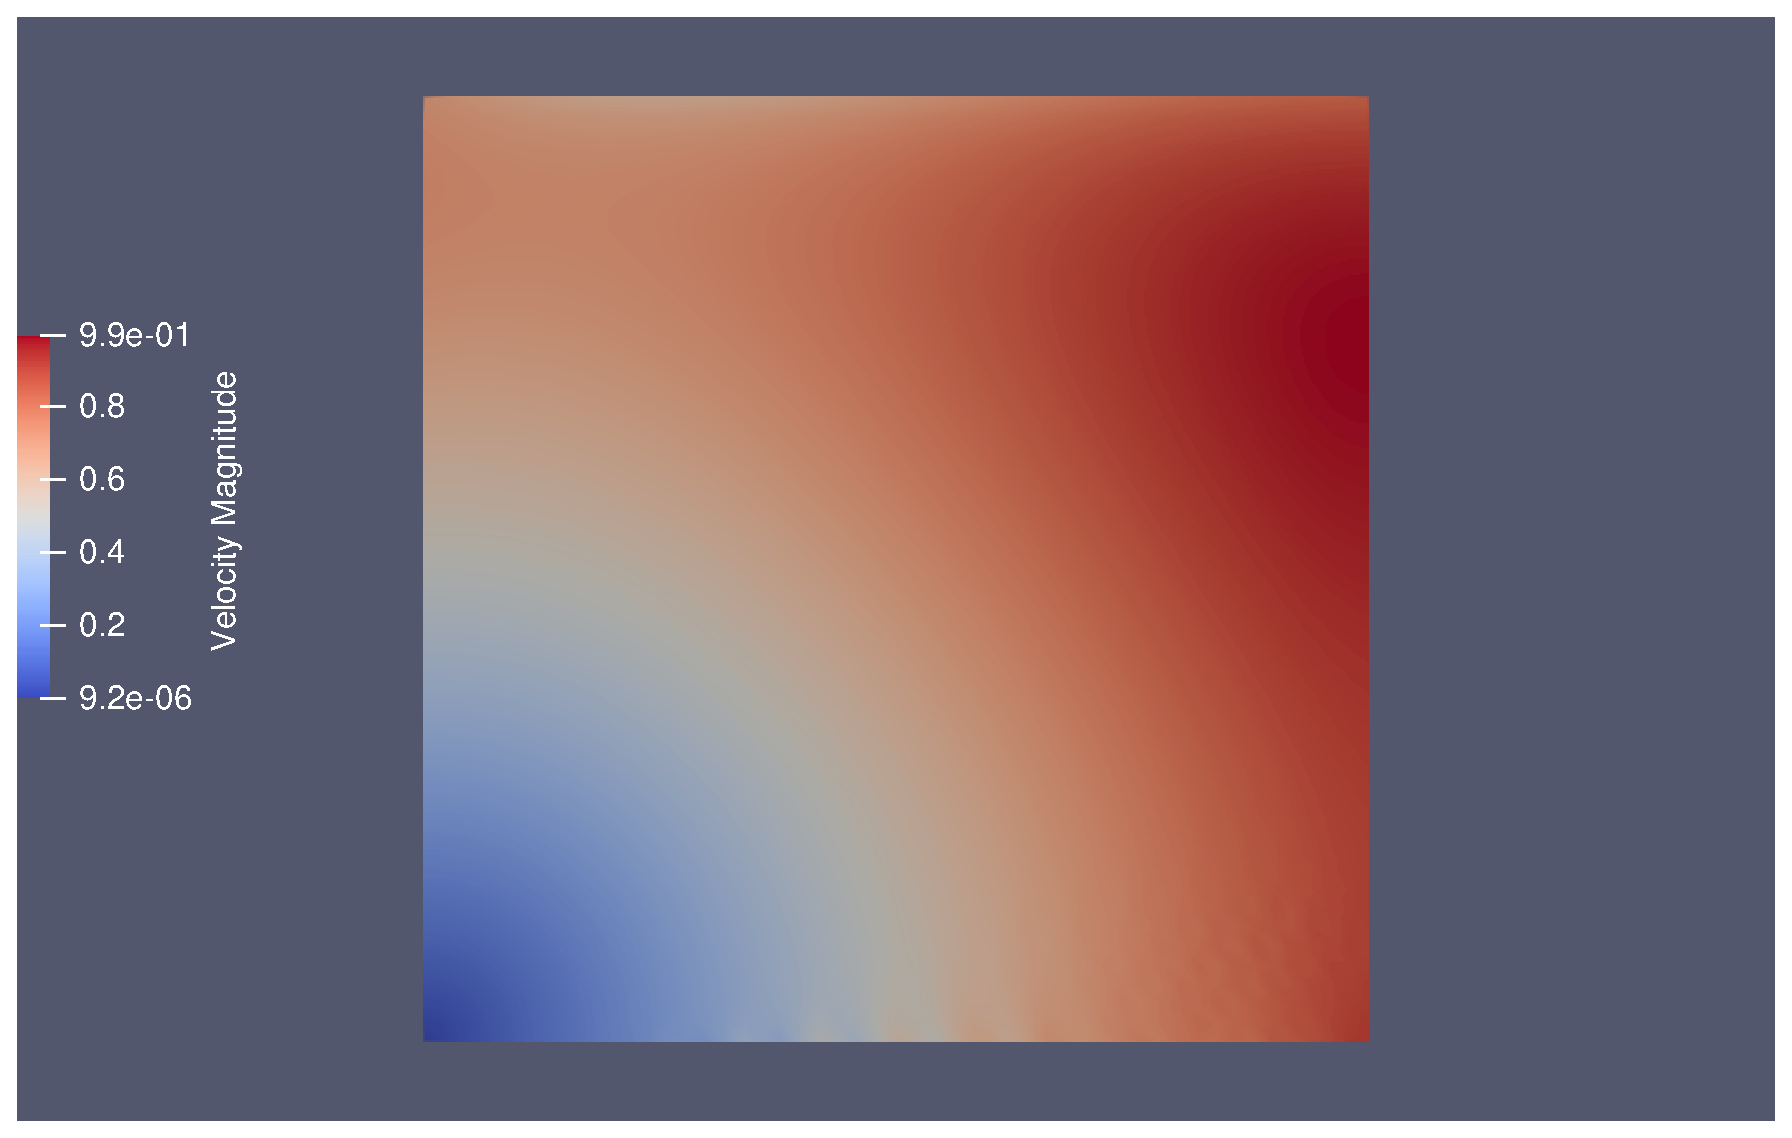
\includegraphics[trim={5cm 0 5cm 0}, clip,width=\textwidth]{./img/75.eps}
        \caption[]%
        {{\small t = 0.75}}
        \label{fig:0.75}
    \end{subfigure}
    \hfill
    \begin{subfigure}[b]{0.475\textwidth}
        \centering
        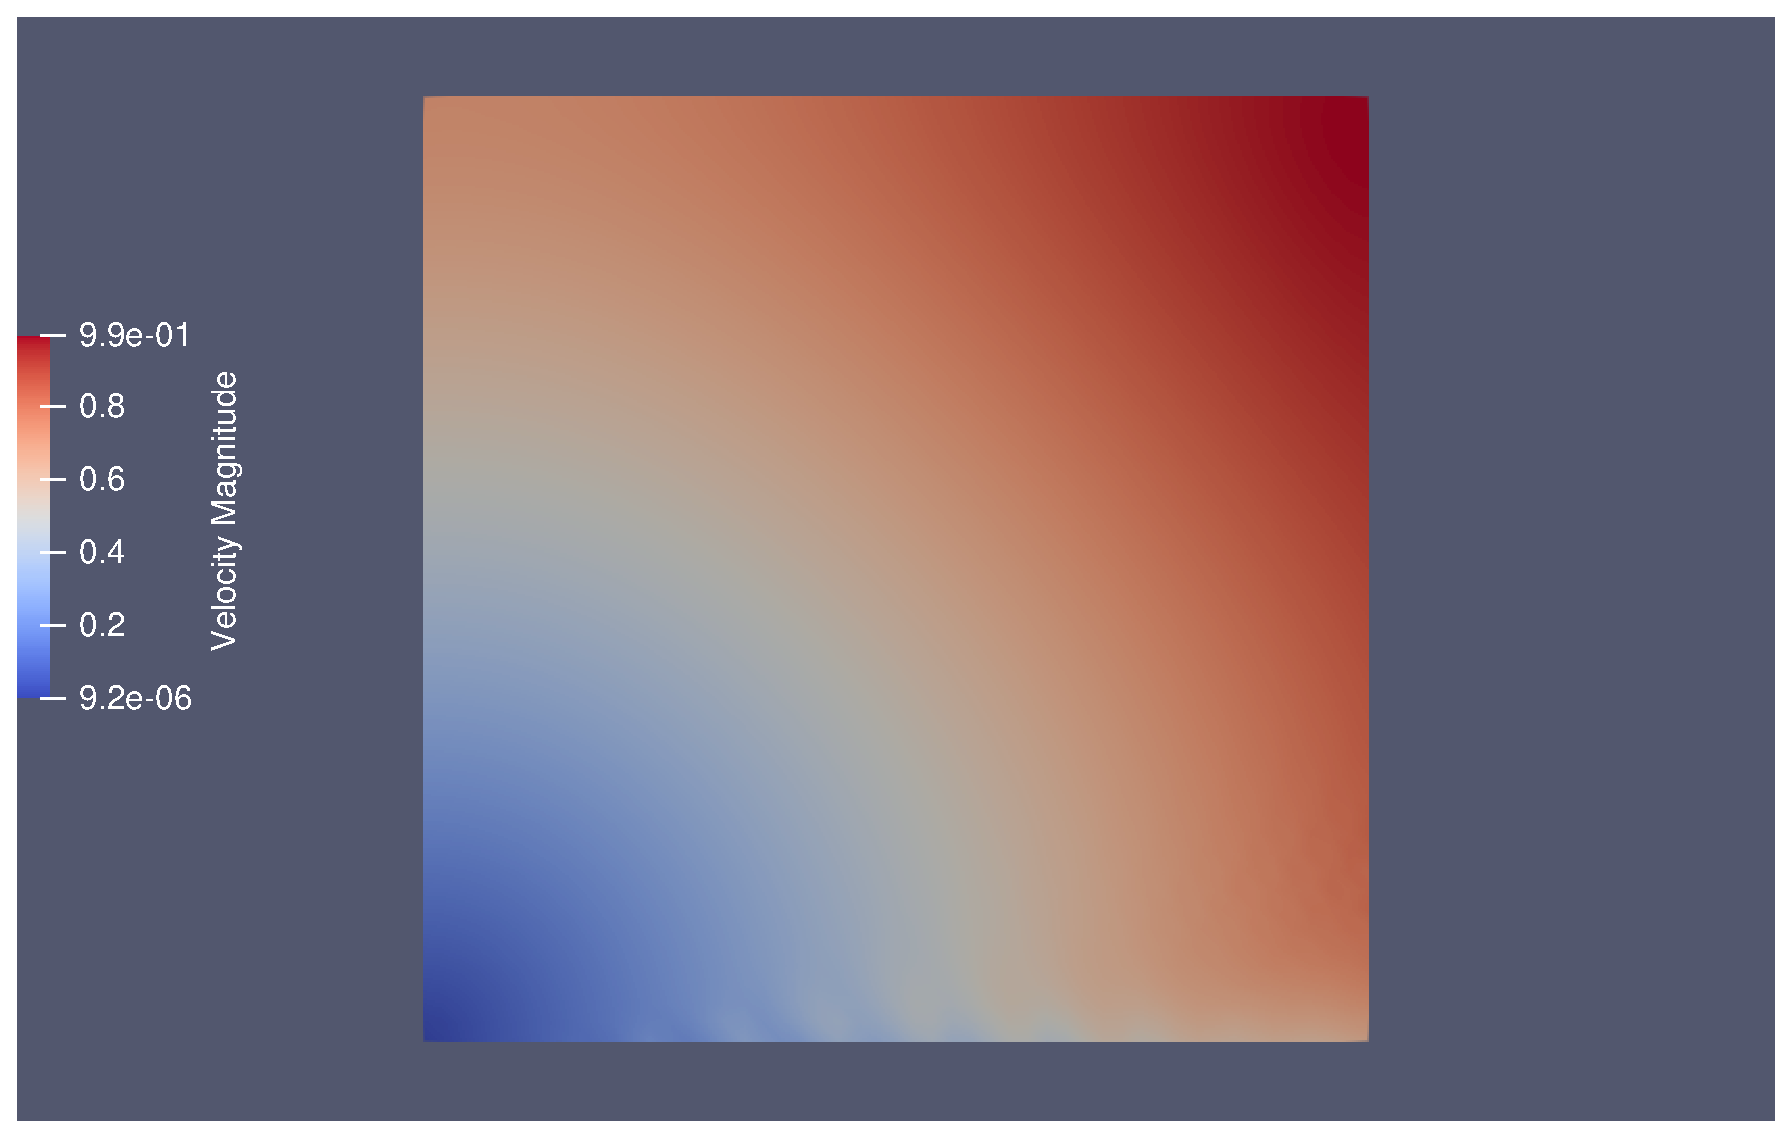
\includegraphics[trim={5cm 0 5cm 0}, clip,width=\textwidth]{./img/100.eps}
        \caption[]%
        {{\small t = 1}}
        \label{fig:1}
    \end{subfigure}
    \caption[ Solution to the Euler Equation using a FEM with L_2 elements ]
    {\small Solution to the Euler Equation using a FEM with Lagrange elements. The colours represent normalised velocity, where blue is $-1$ and red is $1$.}
    \label{fig:Sim}
\end{figure*}
\newpage
\noindent
Unfortunately, the conserved quantities in Figure \ref{fig:conservation} present non-conservation. Due to us using a Crank-Nicholson timestep, which is symplectic, we can say that the error in our scheme comes from our spatial approximation. This is expected as, in general, finite element schemes are not structure-preserving or symplectic. This leads us to search for a new scheme to conserve these quantities. We will overview the theory of structure-preserving numerical methods. \\

\noindent
The idea is as follows: We can discretise the theory presented in this document. Let $F : T^*Q \ti \R \to T^*Q$ be an integrator, where $T^*Q$ is just the tangent space of phase space, manifold, $Q$ and $\R$ is the space where the time steps $h$ live in. Then, we can derive a discrete Euler-Lagrange equation from a discrete Lagrangian $L_d : TQ \ti \R \to \R$ and discrete Hamilton's equations from $H_d : T^*Q\to \R$. Then, we can define the so-called discrete Euler-Lagrange equations. From this, we can discretise into methods in several ways.\\

\noindent
One of the simplest examples of the symplectic method is the midpoint rule. We take a Hamiltonian, $H : T^*Q \to \R$ and define the method for $(p_0,\,q_0) \mapsto (p_1,\,q_1)$ where $z_0 = (p_0,\,q_0)$ and $z_1 = (p_1,\,q_1)$. Then, we define,
$$ \frac{z_1-z_0}{h} = X_H \left( \frac{z_0 + z_1}{2} \right). $$
Then, in the Lagrangian setup, we define the discrete midpoint Lagrangian as,
$$ L_d^{1/2} (q_1,\,q_0,\, h) = hL\left(\frac{q_1 + q_0}{2},\, \frac{q_1 - q_0}{h}\right). $$
Then we can write the scheme as,
\begin{align*}
  \frac{p_1 - p_0}{h} = \pd L {q} \left(\frac{q_1 + q_0}{2},\, \frac{q_1 - q_0}{h}\right) \\
  \frac{p_1 + p_0}{2} = \pd L {\dot q}\left(\frac{q_1 + q_0}{2},\, \frac{q_1 - q_0}{h}\right).
\end{align*}
\noindent
This can be used for our system,
$$ L = H = \frac{1}{2}\int_M |\dot \eta|^2 \mu. $$
This, unfortunately, leaves us with a rather trivial scheme.
\begin{align*}
  p_{k+1} = p_k \\
  q_{k+1} = q_k + hp_k.
\end{align*}
where $q_i$ increases by a fixed step. A similar scheme is derived from a St\"ormer-Verlet scheme. Hence, we need something more complicated. A multisymplectic scheme. This, again, is an area that branches further than this thesis. They are methods that provide discrete conservation laws that agree with what we have seen in this conservation section. For details, see Bridges' paper~\cite{hamil_pdes}.

